\section{Model} \label{sec:model}
In this section, we describe our model in detail. Section \ref{sec:NeuralNetworkArchitecture} describes the architecture of the neural network. Section \ref{sec:Training} describes how the network was trained. Finally, we cover the precision of our model in Section \ref{sec:modelPrecision}.

\subsection{Neural Network Architecture}\label{sec:NeuralNetworkArchitecture}
The model is an attention-based model based on Code2Vec \cite{alon2019code2vec} whereby the overwhelming majority of the weights are in the embedding layer of the network. The architecture of the model has been depicted in Figure \ref{fig:networkArchitecture}. The model takes a set of at most $200$ integer token tuples of the format $(terminal_i, path, terminal_j)$ as an input. It embeds these inputs into a vector with $128$ parameters, whereby the terminal tokens and the path tokens each have their own embedding layer. These embeddings are concatenated into a single vector and passed through a dropout layer. These $200$ vectors are then combined  into a single context vector using an attention mechanism. The context vector will be used to make the final prediction. 

Our model's architecture is similar to the architecture of the original Code2Vec model \cite{alon2019code2vec}. The only difference is in the final layer where our model uses Sigmoid activation with a single output unit. This is because we have a binary classification problem instead of a multi-classification problem. We chose to use the same architecture as Code2Vec to allow the use of transfer learning using the pre-trained weights of Code2Vec \cite{alon2019code2vec}. This also allows us to verify the claim made by the Code2Vec authors that there are a plethora of
programming language processing tasks that their model can be used for \cite{alon2019code2vec}.


\begin{figure*}[b] 
  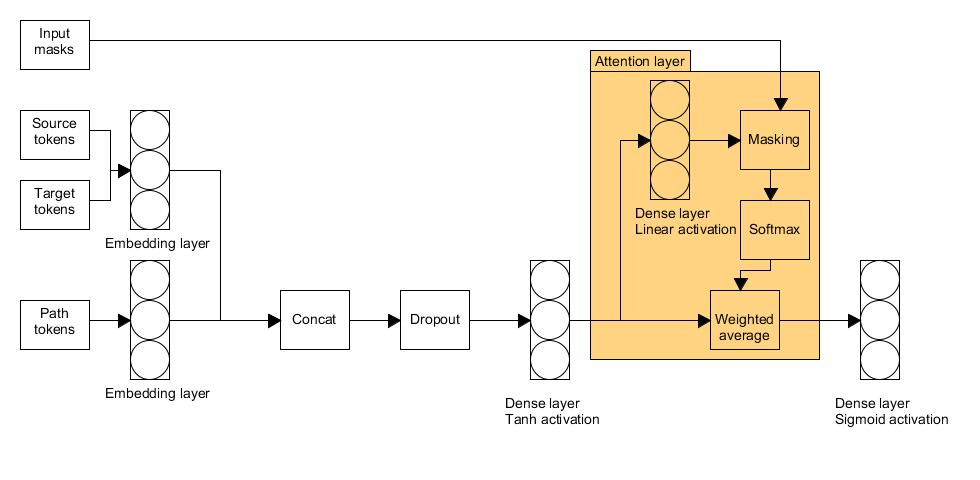
\includegraphics[width=\textwidth,height=7cm]{figures/network.jpg}
  \caption{Neural network architecture}
  \label{fig:networkArchitecture}
\end{figure*}



\subsection{Training}\label{sec:Training}
For the training and validation process, we preprocessed the raw Java training and validation dataset collected by Alon et al. \cite{code2seq}. The generation process resulted in a training set of $1,512,785$ data points (mutated or correct Java methods) and a validation set of $28,086$ data points that were used to train and test our model respectively. We used large over the medium dataset \cite{code2seq} because it resulted in slightly higher overall scores (Table \ref{tab:evaluationDataset}). 
For this training process, we used binary cross-entropy as our loss function and Adam \cite{kingma2014adam} as our optimization algorithm. The model was also trained using early stopping on the validation set. The training process was halted after the accuracy on the validation set did not increase for $2$ Epochs and the weights with the lowest validation loss were kept.

The authors of Code2Vec have speculated that their pre-trained weights could be used for transfer learning \cite{alon2019code2vec}. That is why we experimented with applying transfer learning in two ways. Firstly, we attempted Feature Extraction whereby the pre-trained weights of the Code2Vec model were frozen and only the final layer was replaced and made trainable. Secondly, we tried Fine-Tuning with pre-trained weights of the Code2Vec model as the initial value of our model and allowed the model to update all the values as it saw fit, expect the embeddings weights. Finally, we also trained a model with randomly initialized weights as a baseline. The resulting accuracies are displayed in table \ref{tab:evaluationArchitectures}.



\begin{table}[]
\begin{tabular}{@{}lllll@{}}
\toprule
Model     & \multicolumn{1}{c}{\begin{tabular}[c]{@{}c@{}}Feature\\ Extraction\end{tabular}} & \multicolumn{1}{c}{Fine-Tuning} & \multicolumn{1}{c}{\begin{tabular}[c]{@{}c@{}}Randomly\\ Initialized\end{tabular}} & \multicolumn{1}{c}{\begin{tabular}[c]{@{}c@{}}Transformer \\ model\end{tabular}} \\ \midrule
Accuracy  & 0.732                                                                            & 0.788                           & \textbf{0.790}                                                                     & 0.717                                                                            \\
F1        & 0.709                                                                            & \textbf{0.781}                  & 0.777                                                                              & 0.674                                                                            \\
Precision & 0.776                                                                            & 0.809                           & \textbf{0.831}                                                                     & 0.794                                                                            \\
Recall    & 0.653                                                                            & \textbf{0.756}                  & 0.730                                                                              & 0.585                                                                            \\ \bottomrule
\end{tabular}
\caption{Evaluation comparison of different architectures on an unseen test of $88,228$ examples based on the mutated test set from Alon et al. \cite{code2seq}}
\label{tab:evaluationArchitectures}
\end{table}

\begin{table}[]
\centering
\begin{tabular}{@{}lll@{}}
\toprule
Model     & \begin{tabular}[c]{@{}l@{}}Fine-Tuning\\ medium dataset\end{tabular} & \multicolumn{1}{c}{\begin{tabular}[c]{@{}c@{}}Fine-Tuning\\ large dataset\end{tabular}} \\ \midrule
Accuracy  & 0.758                                                                & \textbf{0.788}                                                                          \\
F1        & 0.757                                                                & \textbf{0.781}                                                                          \\
Precision & 0.762                                                                & \textbf{0.809}                                                                          \\
Recall    & 0.751                                                                & \textbf{0.756}                                                                          \\ \bottomrule
\end{tabular}
\caption{Evaluation comparison of the medium data set  ($482,138$ training examples) and the large data set ($1,512,785$ training examples)  \cite{code2seq} .}
\label{tab:evaluationDataset}
\end{table}


\subsection{Alternative Architecture}\label{sec:AlternativeNeuralNetworkArchitecture}
Besides the original Code2Vec architecture, we also tried a more complicated architecture based on BERT \cite{bertdevlin2018bert}. The idea behind this architecture was that the power of the Code2Vec \cite{alon2019code2vec} architecture lays in the attention mechanism. To verify this idea we tried a transformer model based on BERT. This model encodes the source cod,e in the same manner as the Code2Vec model. It then embeds these input tokens using the frozen pre-trained embedding layers from Code2Vec. Finally, it passes these embedding through multiple BERT layers before making the final prediction. 
However as can be seen in Table \ref{tab:evaluationArchitectures}, this architecture achieved a much lower overall score than the original Code2Vec architecture. This is most likely due to the observed Java code AST being limited to method scope as mentioned in Section \ref{sec:data}. Since our preprocessing is highly depended on the Code2Vec preprocessing pipeline and the overall scores for this model were lower, we did not pursue this architecture any further.

\subsection{Predicting Bug Location}\label{sec:modelPrecision}
Our model looks for bugs with a method-level precision, that is, it predicts whether a method contains an off-by-one bug or not. It is not able to detect where exactly inside that method the bug is. This is due to our effort to capture the context of the whole method. Looking at a smaller section of code would yield more precisely located bugs, but possibly at the cost of context which would reduce the accuracy of the model.